\documentclass{article}
\usepackage{graphicx} % Required for inserting images

\title{Data Analytics Assignment 2 Report}
\author{Aditya Manjunatha }
\date{Btech 22140}

\begin{document}

\maketitle

\section{Image for description}

\begin{figure}[htbp]
  \centering
  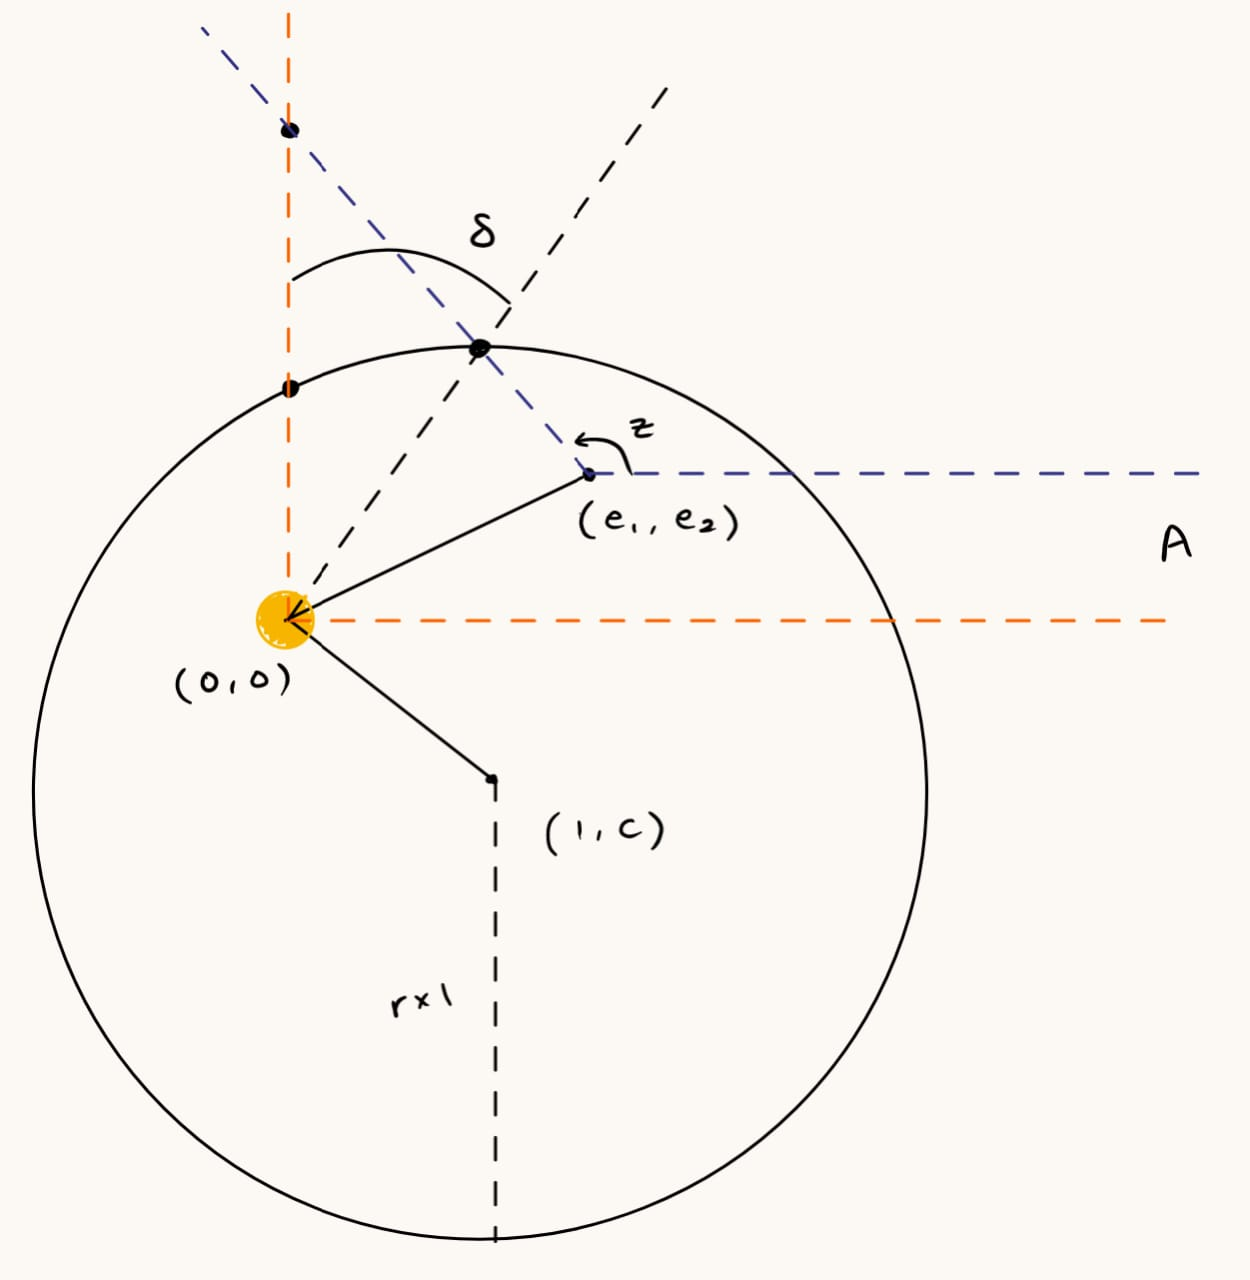
\includegraphics[width=\linewidth]{Image.jpeg}
  \caption{Diagram Visualization}
  \label{fig:example}
\end{figure}

\section{Code Description}
I am briefly decribing what im doing in each of the following functions :
\subsection{days\_between\_dates(date1, date2)}
This function takes two dates as input, where each date is characterized by a tuple of the form (year, month, day, hour, minute). The function returns the number of days between the two dates. The number of days will be fractions becuase we are converting the hours and minutes also into days.

\subsection{get\_times(data)}
As mentioned in the template, this function finds the time at which each opposition happened wrt the first opposition. \\The output given by this fucntion is :-

[0.0, 770.1020833333333, 1534.7381944444444, 2299.2444444444445, 3069.2027777777776, 3854.258333333333, 4663.663888888889, 5459.9638888888885, 6234.592361111111, 7000.521527777778, 7764.529166666666, 8531.619444444445]

\subsection{get\_oppositions(data)}
This function as mentioned in the template returns the longitudes of mars from the sun during each of the oppositions in degrees.\\ The output given by this fucntion is :-

[66.47638888888889, 106.92500000000001, 141.60277777777776, 175.71666666666667, 214.38333333333333, 266.71666666666664, 342.26666666666665, 47.52777777777778, 92.46666666666667, 128.63333333333333, 162.45, 198.61944444444444]

\subsection{calculate\_equant\_longitude\_of\_opp(times, z, s)}
This function returns the longitudes of mars during oppositions wrt to the equant present at (e1, e2).\\
The output of this function is :-

[55.84453273565552, 99.43963256898883, 140.1701256801, 180.8325611800999, 224.35232451343313, 275.78424006898877, 339.97750362454417, 37.302407624543775, 83.2696973467664, 124.67785501343315, 165.0789784023218, 207.0956511801005]
\newpage
\subsection{point\_of\_int\_btw\_equant\_longitude\_and\_orbit(equant\_longitudes, r, c, e1, e2)}
This function returns the point of intersection between the orbit of mars and the equant longitude line for a given opposition as shown in the figure it is the red point.\\
I have done this by substituting the equation of the equant longitude line (which is characterized by the point-slope form of a line where the angle is the equant longitudes and the point on the line is the equant itself)\\
I then substituted this equation into the equation of the orbit, which is a circle that is characterized by the center and the radius.\\
I got a quadratic equation and then solved it to get the point of intersection.\\
I have appropriately rejected the points whenever the line intersected the circle at 2 points.\\

\subsection{point\_of\_int\_btw\_sun\_longitude\_and\_orbit(longitudes, r, c)}
Similar to the previous function i have found the point of intersection between the longitude line from the sun for a given opposition and the orbit.

\subsection{objective\_function(params, times, oppositions)}
This function returns the sum of the squares of the errors .
I have asked it to return this and not the maxError in the error array because this helps us to escape the local minima problem.

\subsection{plot\_orbit\_and\_points()}
This plots all the 24 longitude lines. 12 from the sun and 12 from the equant. We also show where these lines intersect with the orbit. \\

\subsection{MarsEquantModel()}
This function as given in the template returns the error array along with the maximum element in that array.

\subsection{grid\_search()}
This function takes in input the different ranges for the parameters over which you want to search. Uses 5 forloops to find the best parameters which minimize the error.\\

\subsection{bestMarsOrbitParams()}
This function is divided into 2 parts.\\
First we do a coarse search over a specific range as mentioned in the code.\\
Then we use the scipy.optimize minimize function which optimizes our objective\_function . More details on its implementation later.\\
So what i have done is first get an initial guess of the best parameters using the coarse search which is OPTIMIZES THE MAXERROR, then i feed this as the initial guess to the scipy function. The scipy function then takes over and finds the best parameters in the specified bounds which minimizes the OBJECTIVE FUNCTION as mentioned before.
\newpage
\section{Output}
NOTE :- In this code i have not done a COMPLETE EXHAUSTIVE search over every possible value for the parameters, i have narrowed it down as mentioned in the code. Initially when I ran the code , it was taking a lot of time to run, so i did many broad searches and found that the best parameters lie in these ranges. So then i directly ran the loops over these ranges.\\
\vspace{3pt}
\\
After running the bestMarsOrbitParams() function we get the following output BEFORE USING THE SCIPY FUCNTION :-
% c = 155.0, e1 = 1.5, e2 = 149.5, z = 56.0, r = 8.1, s = 0.5240174672489083

\begin{itemize}
    \item c = 151.5
    \item e1 = 1.5
    \item e2 =149.5
    \item z = 56
    \item r = 8.1
    \item s = 0.5240174672489083
    \item error =[-0.2185926287349247, -0.17454674707781237, -0.1534549548056816, -0.16860662589169806, -0.19645290475091315, 0.0887930382491362, 0.2538667972449389, 0.09096558546998779, 0.1319155326884669, 0.1748981085360981, 0.188321546992114, 0.14446761500687444]

    \item max\_error = 0.2538667972449389

\end{itemize}

Then we feed these SUB-OPTIMAL PARAMETERS to the scipy function to get the best parameters.\\
%c = 148.86235336862813, e1 = 1.628748113664418, e2 = 148.93048954942515, z = 55.84453273565552, r = 8.767454193311861, s = 0.52408

\begin{itemize}
    \item best\_c = 148.86235336862813
    \item best\_e1 = 1.628748113664418
    \item best\_e2 = 148.93048954942515
    \item best\_z = 55.84453273565552
    \item best\_s = 0.52408
    \item best\_r = 8.767454193311861
    \item best\_error = [0.03398422660406197, -0.01564999789287924, -0.023955304810471034, 0.0025391298752879266, -0.03127483488324856, 0.015270398626583415, -0.006410870876962349, -0.015595958096810136, -0.0035311303215337375, 0.00012035674799903973, 0.03772763898763287, 0.0067721788963410745]

    \item best\_max\_error = 0.03772763898763287

\end{itemize}

\newpage
\section{The Plots :-}

This is the plot we get after doing the manual coarse search.
\begin{figure}[htbp]
    \centering
    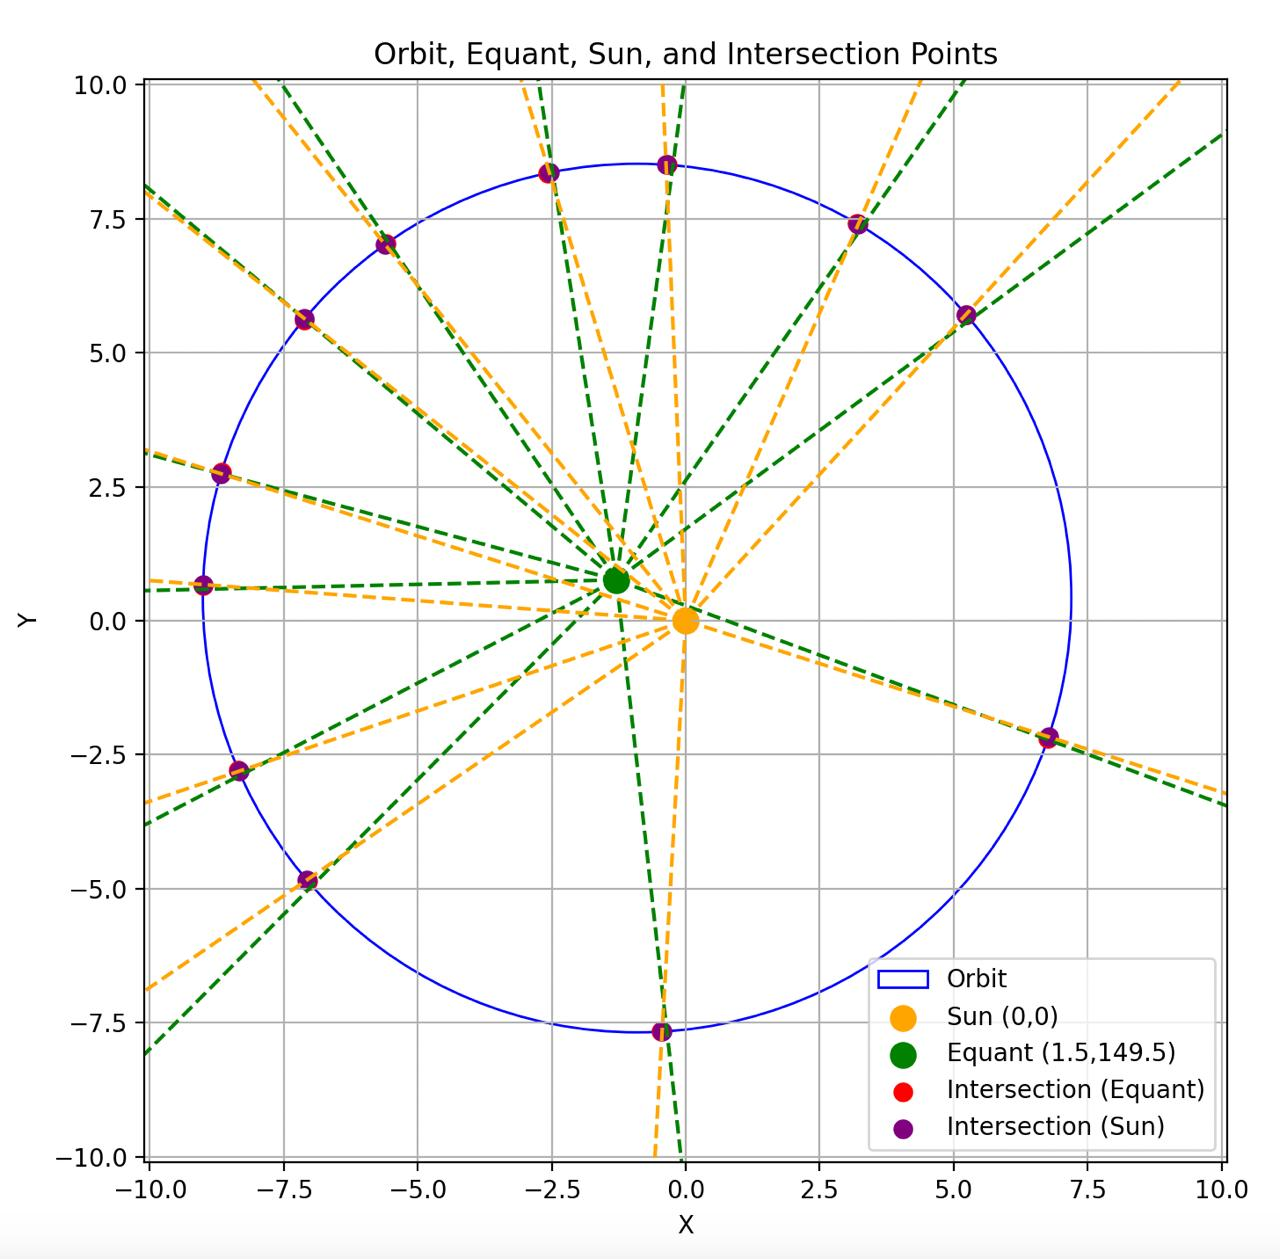
\includegraphics[width=\linewidth]{Before_scipy.jpeg}
    \caption{Plot after Scipy}
    \label{fig1:example}
  \end{figure}

\newpage

This is the plot we get after applying the scipy function.
\begin{figure}[htbp]
    \centering
    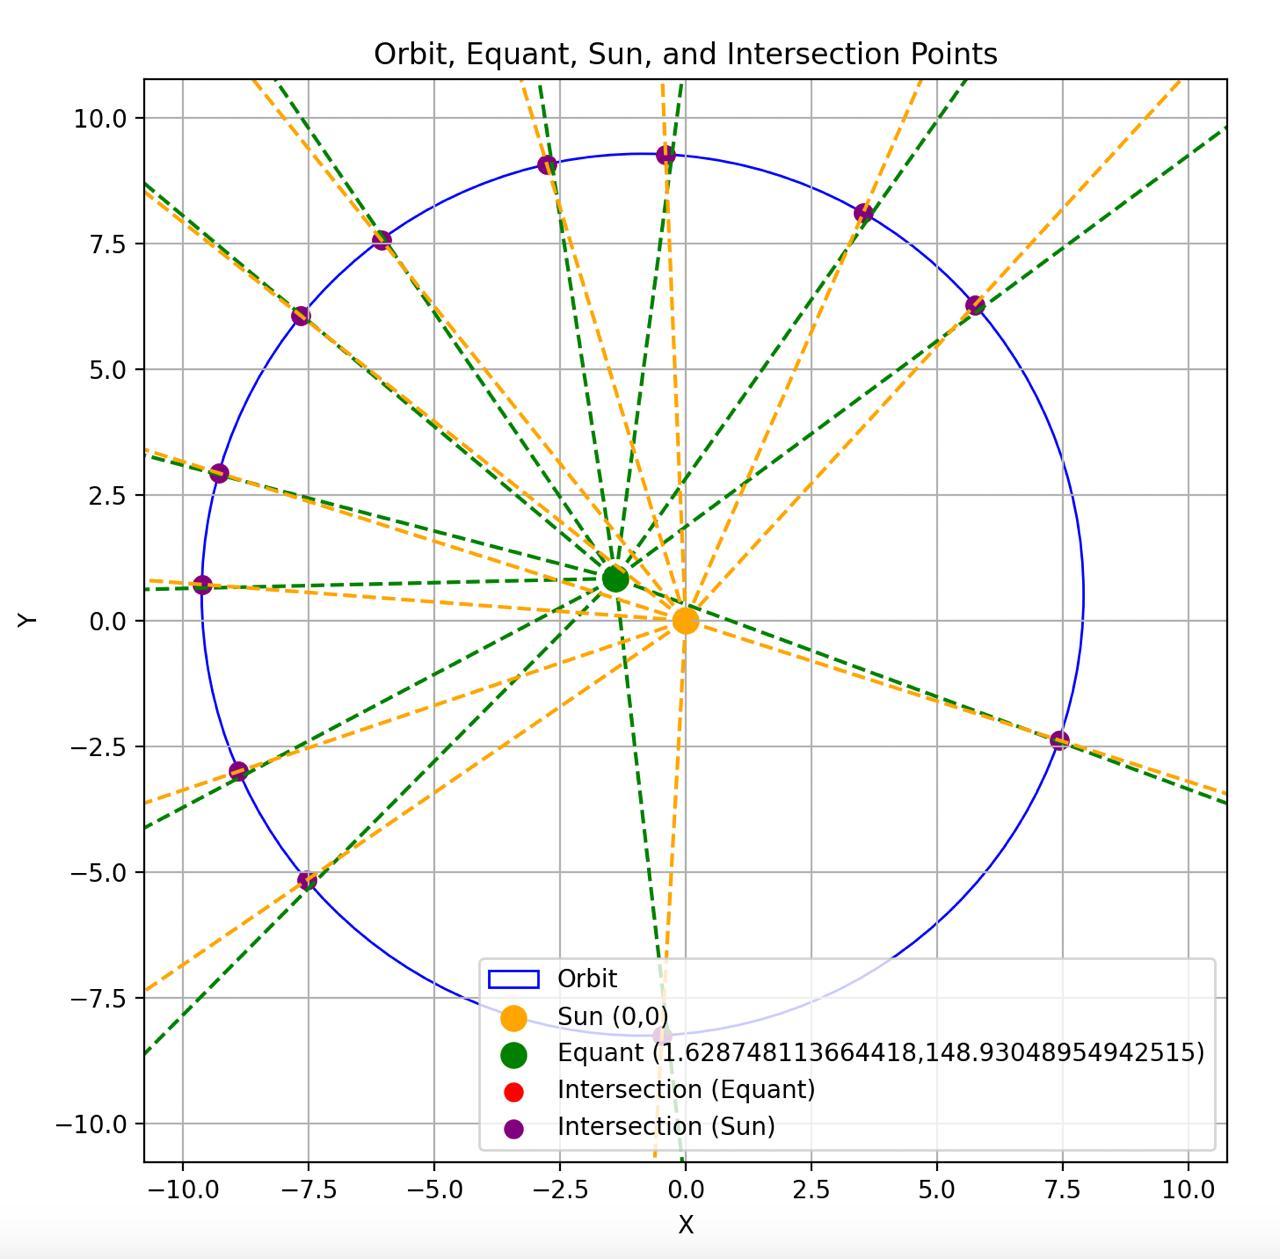
\includegraphics[width=\linewidth]{After_scipy1.jpeg}
    \caption{Plot after Scipy}
    \label{fig2:example}
  \end{figure}

\end{document}
